\section{Galactic Halo Models}
\label{sec:halo_models}
\graphicspath{{Boosted_dm/}}
Since the boosted dark matter being searched for comes from some interaction of the heavy non-interacting dark matter, it's directional distribution around the galactic center is dependent on the density profile of the dark matter halo around the galactic center.  A general form for the density profile (assumed to be spherically symmetric) from cold dark matter simulations is \cite{Yuksel:2007jx}
\begin{equation}
\rho(r)=\frac{\rho_0}{(r/r_s)^\gamma [1+(r/r_s)^\alpha]^(\beta-\gamma)/\alpha}
\label{eq:dm_halo_parm}
\end{equation}.



Parameters of Equation \ref{eq:dm_halo_parm} for the NFW \cite{Navarro:1996ce}, Moore \cite{Moore:1999kx}, and Kravtsov \cite{Kravtsov:1998it} halo models are shown in Table \ref{tab:halo_parms}.
\begin{table}[ht]
\begin{tabular}{lcccccc}
\hline\hline
&$\alpha$&$\beta$&$\gamma$&$r_s$&   $\rho_0$ &   $\rho(R_{sc})$ \\
\hline
Moore & 1.5&3&1.5&28&0.0527&0.27\\
NFW&1&3&1&20&0.259&0.3\\
Kravtsov&2&3&0.4&10&0.703&0.37\\
\hline
\end{tabular}

\caption{Halo parameters for NFW, Moore, and Kravtsov models.  The scale radius $r_s$ is in units of [kpc] while the two densities $\rho_0$ and  $\rho(R_{sc})$ are in units of [GeV/cm$^3$].  $R_{sc}$ is the solar circle radius, 8.5 kpc  \cite{Yuksel:2007jx}.}
\label{tab:halo_parms}
\end{table}

The rate of boosted dark matter events coming from the annihilation or decay of dark matter from a particular direction in the sky is proportional to the so called ``J-factor", which is the line of sight integral of dark matter density for decay, or density squared for annihilation, and is a function of the angle between the event direction and the direction to the galactic center:

\begin{equation}
\mathcal{J}_{ann}(\theta_\textrm{GC})=\frac{1}{R_N\rho_N^2}\int\limits_0^{l_\textrm{max}} \rho^2 \left(\sqrt{R_{sc}^2-2lR_{sc}\cos{\theta_\textrm{GC}}+l^2}\right)dl\\
\label{eqn:J_ann}
\end{equation}
\begin{equation}
\mathcal{J}_{decay}(\theta_\textrm{GC})=\frac{1}{R_N\rho_N}\int\limits_0^{l_\textrm{max}} \rho \left(\sqrt{R_{sc}^2-2lR_{sc}\cos{\theta_\textrm{GC}}+l^2}\right)dl
\label{eqn:J_d}
\end{equation}
where $\theta_{GC}$ is the angle to the Galactic Center and $R_{sc}$ is the solar circle radius (8.5 kpc).  The upper limit of integration $l_\textrm{max}$ is defined by by the adopted halo size $R_{\textrm{MW}}$:
\begin{equation}
l_\textrm{max}=\sqrt{R^2_\textrm{MW}-R^2_{sc}\sin^2 \theta_{GC}} + R^2_{sc}\cos{\theta_{GC}}.
\label{eqn:l_max}
\end{equation}
While the halo size $R_{\textrm{MW}}$ appears to be an additional important parameter, $\rho$ drops off sharply past 20-30 kpc, as shown if \ref{fig:dm_density}, so that the calculation of $\mathcal{J}$ is insensitive to the choosen value of $R_{\textrm{MW}}$ as long as it is above this range.  The prefactors $\frac{1}{R_N\rho_N^2}$ and $\frac{1}{R_N\rho_N}$ in Equations \ref{eqn:J_ann} and \ref{eqn:J_d} are arbitrary scaling factors used to make $\mathcal{J}$ dimensionless.  Figure \ref{fig:dm_halos} shows the dark matter halo density J factors for the Moore, NFW, and Kravstov models.  The J factors in \ref{fig:dm_J_ann} and \ref{fig:dm_J_d} are calculated with $R_{\textrm{MW}}=40$ kpc and the standard scaling choice of $R_N=R_{sc}=8.5$ kpc, $\rho_N=0.3$ GeV/cm$^3$.  The J factor is taken to be flat at the innermost 0.1$^\circ$ to avoid divergence of $\mathcal{J}$ due to cuspy profiles, which may be an artifact of simulation \cite{Yuksel:2007jx}. 
\begin{figure}
 		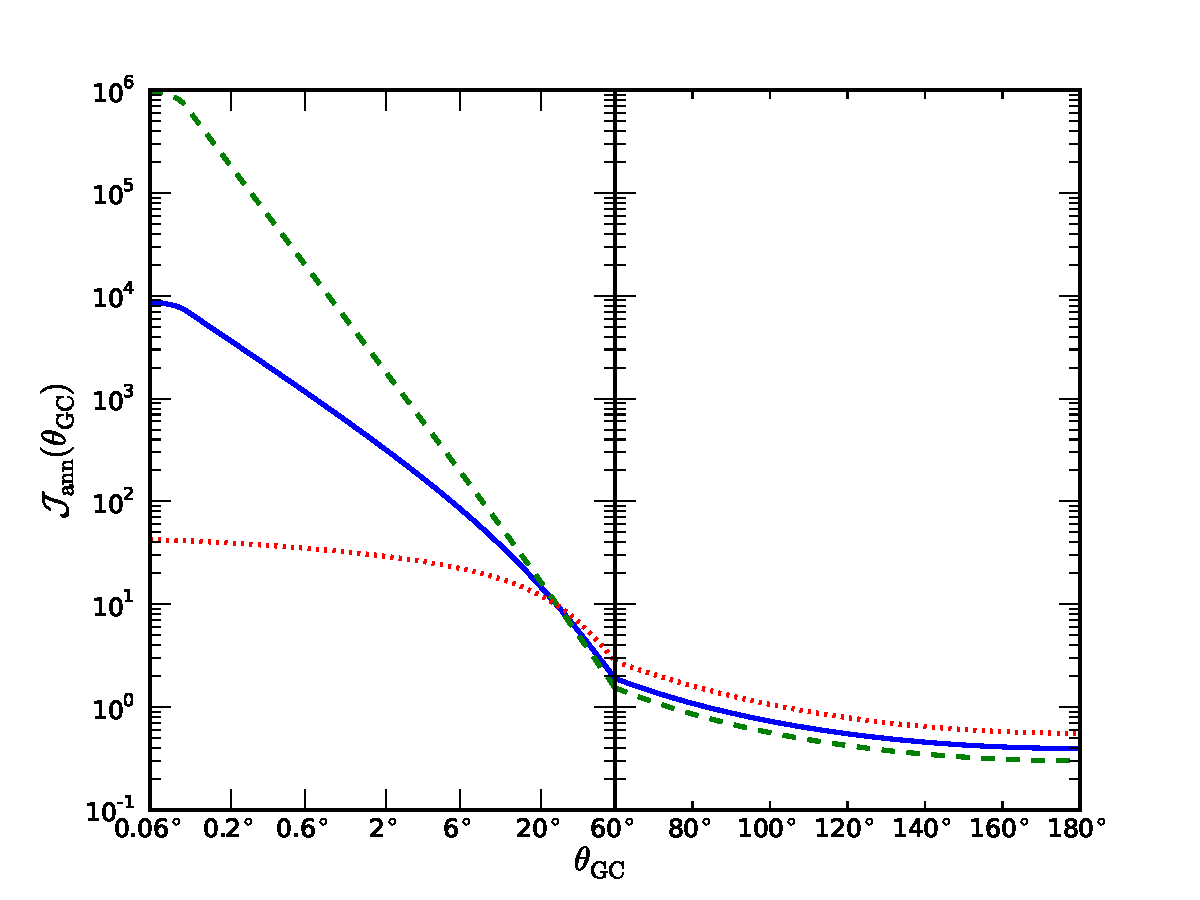
\includegraphics[width=0.4\textwidth]{figures/DM_J_ann.pdf}
		\label{fig:dm_density}
\caption{stuff}
\end{figure}
\begin{figure}
	\centering
	\subfigure[]{
 		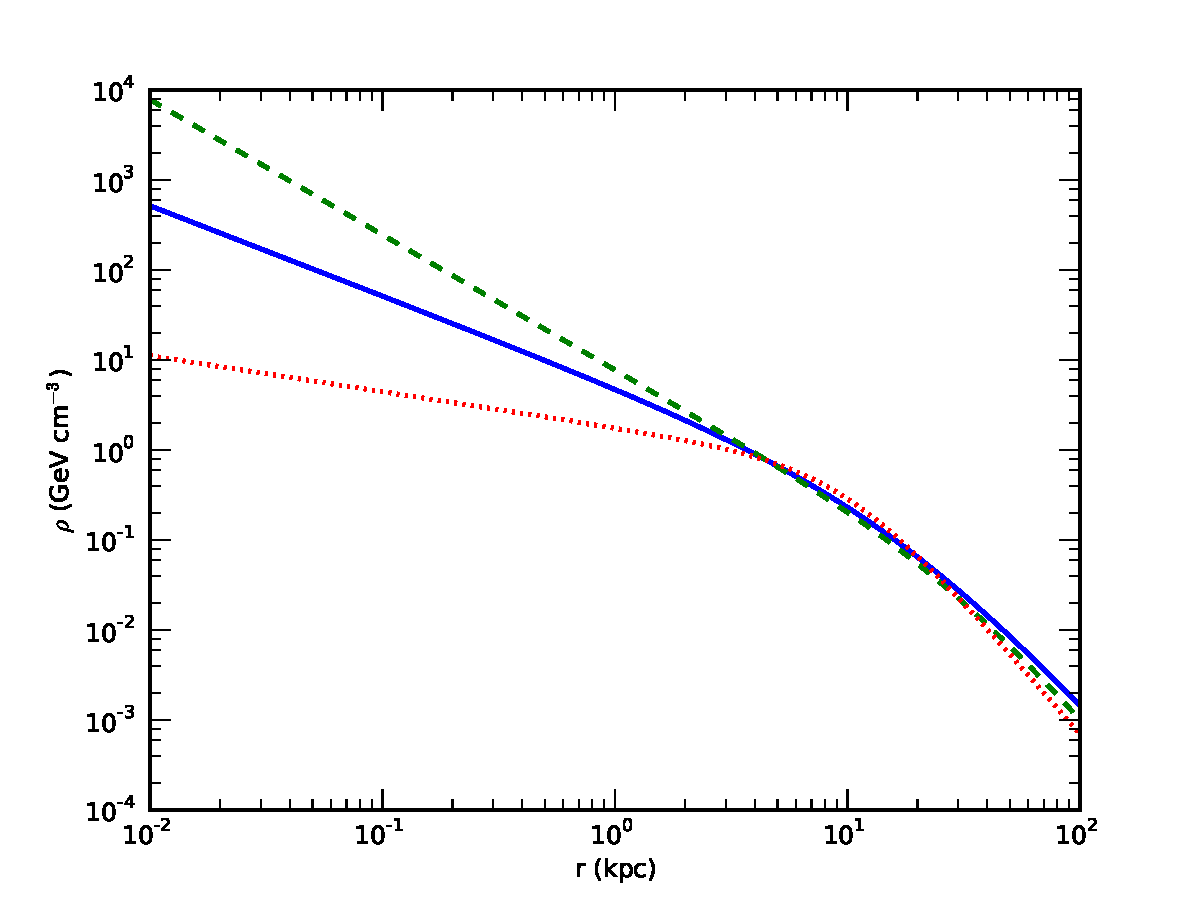
\includegraphics[width=0.4\textwidth]{figures/DM_Halo_density.pdf}
		\label{fig:dm_density}
	}
	\subfigure[]{
 		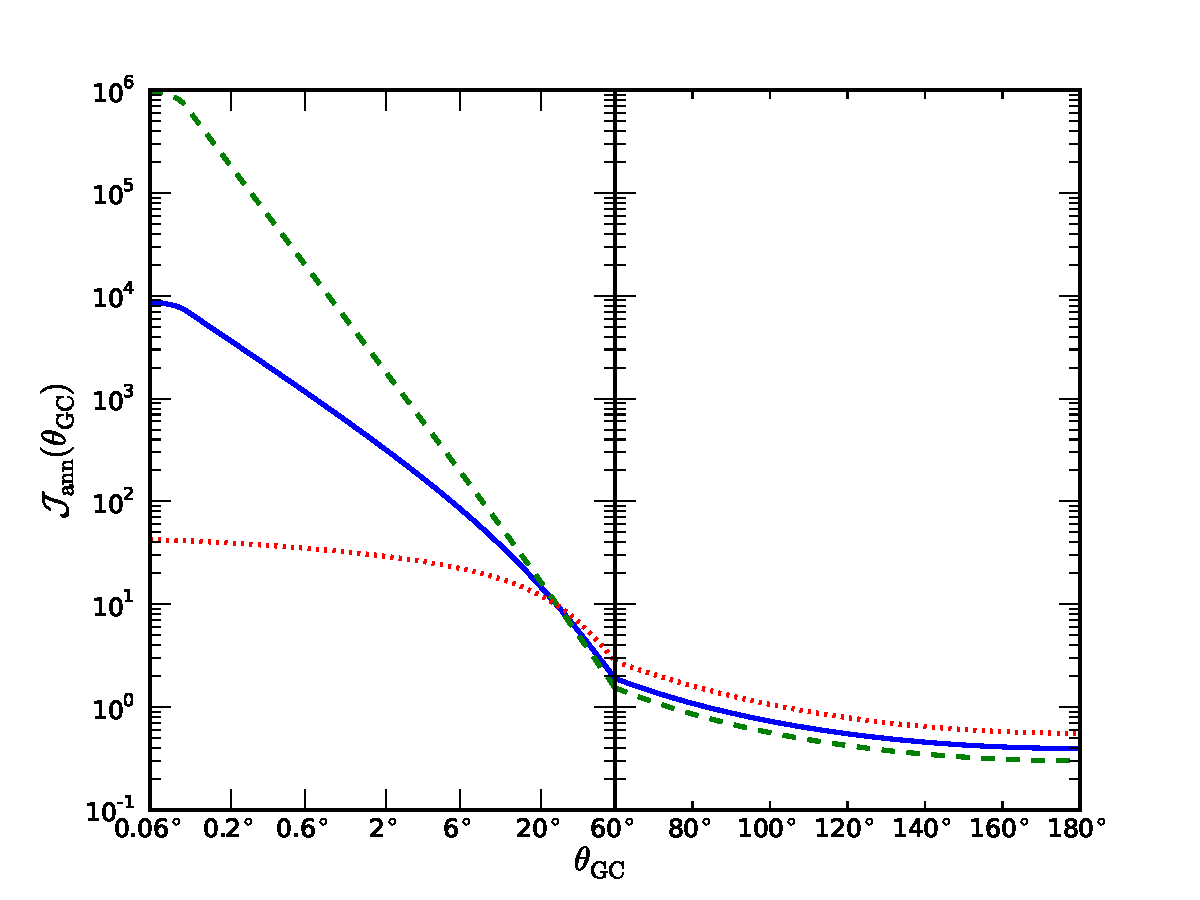
\includegraphics[width=0.4\textwidth]{figures/DM_J_ann.pdf}
		\label{fig:dm_J_ann}
	}	
	\subfigure[]{
 		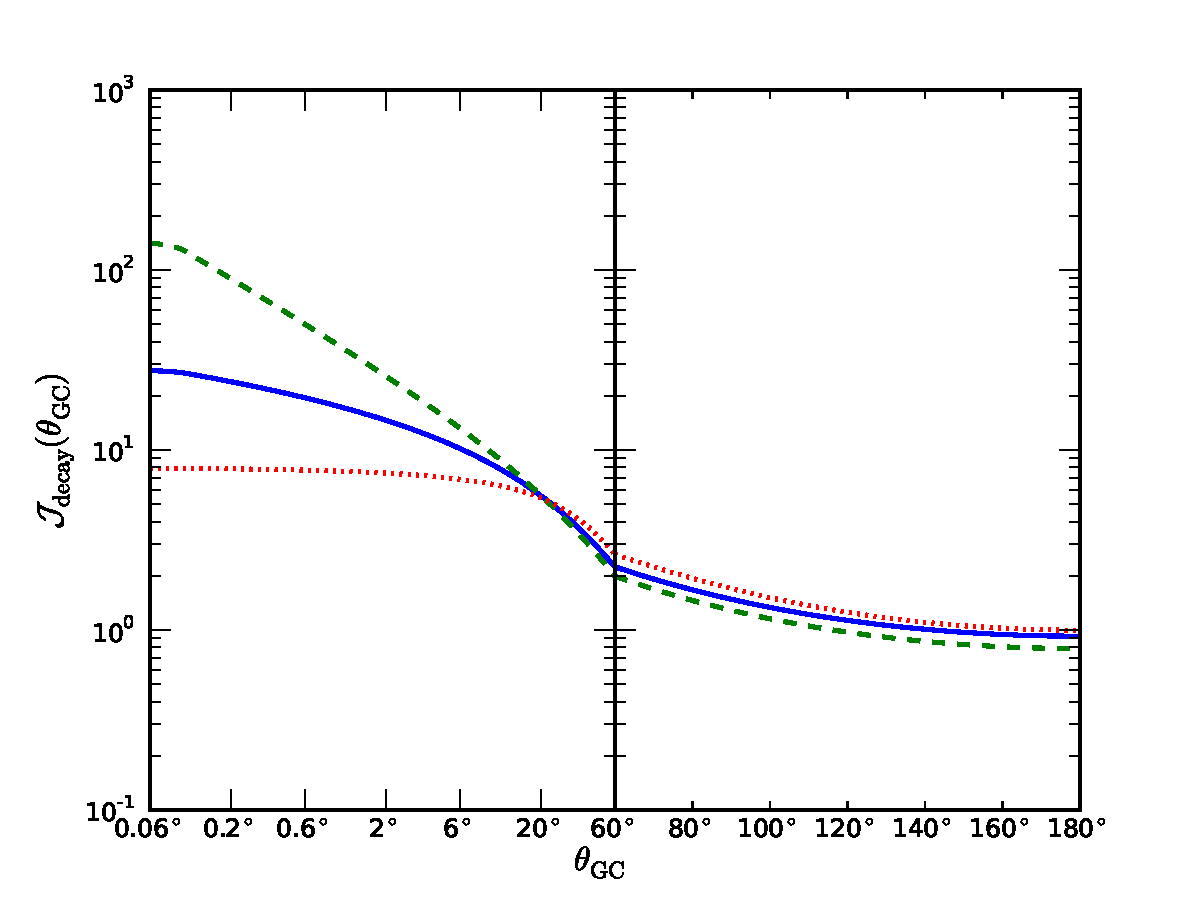
\includegraphics[width=0.4\textwidth]{figures/DM_J_decay.pdf}
		\label{fig:dm_J_d}
	}	
\caption{Moore (dashed green), NFW (solid blue) and Kravstov (dotted red) dark matter halo models.  \ref{fig:dm_density} shows the dark matter density as a function of distance from the galactic center.   \ref{fig:dm_J_ann} and \ref{fig:dm_J_d} show the J factors for the product of annihilating and decaying dark matter as a function of angle from the galactic center.  Note that the x-axis is logarithmic on the left and linear on the right of \ref{fig:dm_J_ann} and \ref{fig:dm_J_d}.}
\label{fig:dm_halos}
\end{figure} 
